\documentclass[twoside]{book}

% Packages required by doxygen
\usepackage{fixltx2e}
\usepackage{calc}
\usepackage{doxygen}
\usepackage[export]{adjustbox} % also loads graphicx
\usepackage{graphicx}
\usepackage[utf8]{inputenc}
\usepackage{makeidx}
\usepackage{multicol}
\usepackage{multirow}
\PassOptionsToPackage{warn}{textcomp}
\usepackage{textcomp}
\usepackage[nointegrals]{wasysym}
\usepackage[table]{xcolor}

% Font selection
\usepackage[T1]{fontenc}
\usepackage[scaled=.90]{helvet}
\usepackage{courier}
\usepackage{amssymb}
\usepackage{sectsty}
\renewcommand{\familydefault}{\sfdefault}
\allsectionsfont{%
  \fontseries{bc}\selectfont%
  \color{darkgray}%
}
\renewcommand{\DoxyLabelFont}{%
  \fontseries{bc}\selectfont%
  \color{darkgray}%
}
\newcommand{\+}{\discretionary{\mbox{\scriptsize$\hookleftarrow$}}{}{}}

% Page & text layout
\usepackage{geometry}
\geometry{%
  a4paper,%
  top=2.5cm,%
  bottom=2.5cm,%
  left=2.5cm,%
  right=2.5cm%
}
\tolerance=750
\hfuzz=15pt
\hbadness=750
\setlength{\emergencystretch}{15pt}
\setlength{\parindent}{0cm}
\setlength{\parskip}{3ex plus 2ex minus 2ex}
\makeatletter
\renewcommand{\paragraph}{%
  \@startsection{paragraph}{4}{0ex}{-1.0ex}{1.0ex}{%
    \normalfont\normalsize\bfseries\SS@parafont%
  }%
}
\renewcommand{\subparagraph}{%
  \@startsection{subparagraph}{5}{0ex}{-1.0ex}{1.0ex}{%
    \normalfont\normalsize\bfseries\SS@subparafont%
  }%
}
\makeatother

% Headers & footers
\usepackage{fancyhdr}
\pagestyle{fancyplain}
\fancyhead[LE]{\fancyplain{}{\bfseries\thepage}}
\fancyhead[CE]{\fancyplain{}{}}
\fancyhead[RE]{\fancyplain{}{\bfseries\leftmark}}
\fancyhead[LO]{\fancyplain{}{\bfseries\rightmark}}
\fancyhead[CO]{\fancyplain{}{}}
\fancyhead[RO]{\fancyplain{}{\bfseries\thepage}}
\fancyfoot[LE]{\fancyplain{}{}}
\fancyfoot[CE]{\fancyplain{}{}}
\fancyfoot[RE]{\fancyplain{}{\bfseries\scriptsize Generated by Doxygen }}
\fancyfoot[LO]{\fancyplain{}{\bfseries\scriptsize Generated by Doxygen }}
\fancyfoot[CO]{\fancyplain{}{}}
\fancyfoot[RO]{\fancyplain{}{}}
\renewcommand{\footrulewidth}{0.4pt}
\renewcommand{\chaptermark}[1]{%
  \markboth{#1}{}%
}
\renewcommand{\sectionmark}[1]{%
  \markright{\thesection\ #1}%
}

% Indices & bibliography
\usepackage{natbib}
\usepackage[titles]{tocloft}
\setcounter{tocdepth}{3}
\setcounter{secnumdepth}{5}
\makeindex

% Hyperlinks (required, but should be loaded last)
\usepackage{ifpdf}
\ifpdf
  \usepackage[pdftex,pagebackref=true]{hyperref}
\else
  \usepackage[ps2pdf,pagebackref=true]{hyperref}
\fi
\hypersetup{%
  colorlinks=true,%
  linkcolor=blue,%
  citecolor=blue,%
  unicode%
}

% Custom commands
\newcommand{\clearemptydoublepage}{%
  \newpage{\pagestyle{empty}\cleardoublepage}%
}

\usepackage{caption}
\captionsetup{labelsep=space,justification=centering,font={bf},singlelinecheck=off,skip=4pt,position=top}

%===== C O N T E N T S =====

\begin{document}

% Titlepage & ToC
\hypersetup{pageanchor=false,
             bookmarksnumbered=true,
             pdfencoding=unicode
            }
\pagenumbering{alph}
\begin{titlepage}
\vspace*{7cm}
\begin{center}%
{\Large Conway \\[1ex]\large 0.\+9 }\\
\vspace*{1cm}
{\large Generated by Doxygen 1.8.12}\\
\end{center}
\end{titlepage}
\clearemptydoublepage
\pagenumbering{roman}
\tableofcontents
\clearemptydoublepage
\pagenumbering{arabic}
\hypersetup{pageanchor=true}

%--- Begin generated contents ---
\chapter{Hierarchical Index}
\section{Class Hierarchy}
This inheritance list is sorted roughly, but not completely, alphabetically\+:\begin{DoxyCompactList}
\item \contentsline{section}{io.\+github.\+chrishengler.\+conway.\+Cell}{\pageref{classio_1_1github_1_1chrishengler_1_1conway_1_1_cell}}{}
\item \contentsline{section}{io.\+github.\+chrishengler.\+conway.\+Cell\+Board}{\pageref{classio_1_1github_1_1chrishengler_1_1conway_1_1_cell_board}}{}
\item \contentsline{section}{io.\+github.\+chrishengler.\+conway.\+Conway}{\pageref{classio_1_1github_1_1chrishengler_1_1conway_1_1_conway}}{}
\item \contentsline{section}{io.\+github.\+chrishengler.\+conway.\+Conway\+App}{\pageref{classio_1_1github_1_1chrishengler_1_1conway_1_1_conway_app}}{}
\item \contentsline{section}{io.\+github.\+chrishengler.\+conway.\+Game}{\pageref{classio_1_1github_1_1chrishengler_1_1conway_1_1_game}}{}
\item J\+Panel\begin{DoxyCompactList}
\item \contentsline{section}{io.\+github.\+chrishengler.\+conway.\+Conway\+Canvas}{\pageref{classio_1_1github_1_1chrishengler_1_1conway_1_1_conway_canvas}}{}
\end{DoxyCompactList}
\item Runnable\begin{DoxyCompactList}
\item \contentsline{section}{io.\+github.\+chrishengler.\+conway.\+Conway\+Canvas}{\pageref{classio_1_1github_1_1chrishengler_1_1conway_1_1_conway_canvas}}{}
\end{DoxyCompactList}
\item Component\+Listener\begin{DoxyCompactList}
\item \contentsline{section}{io.\+github.\+chrishengler.\+conway.\+Conway\+Canvas}{\pageref{classio_1_1github_1_1chrishengler_1_1conway_1_1_conway_canvas}}{}
\end{DoxyCompactList}
\item Mouse\+Listener\begin{DoxyCompactList}
\item \contentsline{section}{io.\+github.\+chrishengler.\+conway.\+Conway\+Canvas}{\pageref{classio_1_1github_1_1chrishengler_1_1conway_1_1_conway_canvas}}{}
\end{DoxyCompactList}
\item Mouse\+Motion\+Listener\begin{DoxyCompactList}
\item \contentsline{section}{io.\+github.\+chrishengler.\+conway.\+Conway\+Canvas}{\pageref{classio_1_1github_1_1chrishengler_1_1conway_1_1_conway_canvas}}{}
\end{DoxyCompactList}
\end{DoxyCompactList}

\chapter{Class Index}
\section{Class List}
Here are the classes, structs, unions and interfaces with brief descriptions\+:\begin{DoxyCompactList}
\item\contentsline{section}{\hyperlink{classio_1_1github_1_1chrishengler_1_1conway_1_1_cell}{io.\+github.\+chrishengler.\+conway.\+Cell} }{\pageref{classio_1_1github_1_1chrishengler_1_1conway_1_1_cell}}{}
\item\contentsline{section}{\hyperlink{classio_1_1github_1_1chrishengler_1_1conway_1_1_cell_board}{io.\+github.\+chrishengler.\+conway.\+Cell\+Board} }{\pageref{classio_1_1github_1_1chrishengler_1_1conway_1_1_cell_board}}{}
\item\contentsline{section}{\hyperlink{classio_1_1github_1_1chrishengler_1_1conway_1_1_conway}{io.\+github.\+chrishengler.\+conway.\+Conway} }{\pageref{classio_1_1github_1_1chrishengler_1_1conway_1_1_conway}}{}
\item\contentsline{section}{\hyperlink{classio_1_1github_1_1chrishengler_1_1conway_1_1_conway_app}{io.\+github.\+chrishengler.\+conway.\+Conway\+App} }{\pageref{classio_1_1github_1_1chrishengler_1_1conway_1_1_conway_app}}{}
\item\contentsline{section}{\hyperlink{classio_1_1github_1_1chrishengler_1_1conway_1_1_conway_canvas}{io.\+github.\+chrishengler.\+conway.\+Conway\+Canvas} }{\pageref{classio_1_1github_1_1chrishengler_1_1conway_1_1_conway_canvas}}{}
\item\contentsline{section}{\hyperlink{classio_1_1github_1_1chrishengler_1_1conway_1_1_game}{io.\+github.\+chrishengler.\+conway.\+Game} }{\pageref{classio_1_1github_1_1chrishengler_1_1conway_1_1_game}}{}
\end{DoxyCompactList}

\chapter{Class Documentation}
\hypertarget{classio_1_1github_1_1chrishengler_1_1conway_1_1_cell}{}\section{io.\+github.\+chrishengler.\+conway.\+Cell Class Reference}
\label{classio_1_1github_1_1chrishengler_1_1conway_1_1_cell}\index{io.\+github.\+chrishengler.\+conway.\+Cell@{io.\+github.\+chrishengler.\+conway.\+Cell}}
\subsection*{Public Member Functions}
\begin{DoxyCompactItemize}
\item 
\hyperlink{classio_1_1github_1_1chrishengler_1_1conway_1_1_cell_aebac2efd98126a93655bcb52043ae158}{Cell} ()
\item 
\hyperlink{classio_1_1github_1_1chrishengler_1_1conway_1_1_cell_ac93c3921810b8440b46384c364dfb941}{Cell} (boolean alive)
\item 
void \hyperlink{classio_1_1github_1_1chrishengler_1_1conway_1_1_cell_afd2b3126a3cac2f77857efaa34fe8ba3}{set\+Alive} (boolean alive)
\item 
void {\bfseries toggle} ()\hypertarget{classio_1_1github_1_1chrishengler_1_1conway_1_1_cell_a30841f0b9b9c4c5b5d2637f0ea9fe197}{}\label{classio_1_1github_1_1chrishengler_1_1conway_1_1_cell_a30841f0b9b9c4c5b5d2637f0ea9fe197}

\item 
boolean \hyperlink{classio_1_1github_1_1chrishengler_1_1conway_1_1_cell_a0b522d80bc26dbd497b5b4192de653eb}{is\+Alive} ()
\end{DoxyCompactItemize}


\subsection{Detailed Description}
\begin{DoxyAuthor}{Author}
Chris Hengler 
\end{DoxyAuthor}


\subsection{Constructor \& Destructor Documentation}
\index{io\+::github\+::chrishengler\+::conway\+::\+Cell@{io\+::github\+::chrishengler\+::conway\+::\+Cell}!Cell@{Cell}}
\index{Cell@{Cell}!io\+::github\+::chrishengler\+::conway\+::\+Cell@{io\+::github\+::chrishengler\+::conway\+::\+Cell}}
\subsubsection[{\texorpdfstring{Cell()}{Cell()}}]{\setlength{\rightskip}{0pt plus 5cm}io.\+github.\+chrishengler.\+conway.\+Cell.\+Cell (
\begin{DoxyParamCaption}
{}
\end{DoxyParamCaption}
)}\hypertarget{classio_1_1github_1_1chrishengler_1_1conway_1_1_cell_aebac2efd98126a93655bcb52043ae158}{}\label{classio_1_1github_1_1chrishengler_1_1conway_1_1_cell_aebac2efd98126a93655bcb52043ae158}
constructor w/o args, default to not alive \index{io\+::github\+::chrishengler\+::conway\+::\+Cell@{io\+::github\+::chrishengler\+::conway\+::\+Cell}!Cell@{Cell}}
\index{Cell@{Cell}!io\+::github\+::chrishengler\+::conway\+::\+Cell@{io\+::github\+::chrishengler\+::conway\+::\+Cell}}
\subsubsection[{\texorpdfstring{Cell(boolean alive)}{Cell(boolean alive)}}]{\setlength{\rightskip}{0pt plus 5cm}io.\+github.\+chrishengler.\+conway.\+Cell.\+Cell (
\begin{DoxyParamCaption}
\item[{boolean}]{alive}
\end{DoxyParamCaption}
)}\hypertarget{classio_1_1github_1_1chrishengler_1_1conway_1_1_cell_ac93c3921810b8440b46384c364dfb941}{}\label{classio_1_1github_1_1chrishengler_1_1conway_1_1_cell_ac93c3921810b8440b46384c364dfb941}
constructor with boolean to set cell alive/not alive


\begin{DoxyParams}{Parameters}
{\em alive} & cell is alive \\
\hline
\end{DoxyParams}


\subsection{Member Function Documentation}
\index{io\+::github\+::chrishengler\+::conway\+::\+Cell@{io\+::github\+::chrishengler\+::conway\+::\+Cell}!is\+Alive@{is\+Alive}}
\index{is\+Alive@{is\+Alive}!io\+::github\+::chrishengler\+::conway\+::\+Cell@{io\+::github\+::chrishengler\+::conway\+::\+Cell}}
\subsubsection[{\texorpdfstring{is\+Alive()}{isAlive()}}]{\setlength{\rightskip}{0pt plus 5cm}boolean io.\+github.\+chrishengler.\+conway.\+Cell.\+is\+Alive (
\begin{DoxyParamCaption}
{}
\end{DoxyParamCaption}
)}\hypertarget{classio_1_1github_1_1chrishengler_1_1conway_1_1_cell_a0b522d80bc26dbd497b5b4192de653eb}{}\label{classio_1_1github_1_1chrishengler_1_1conway_1_1_cell_a0b522d80bc26dbd497b5b4192de653eb}
check whether or not cell is alive

\begin{DoxyReturn}{Returns}
true if cell is alive 
\end{DoxyReturn}
\index{io\+::github\+::chrishengler\+::conway\+::\+Cell@{io\+::github\+::chrishengler\+::conway\+::\+Cell}!set\+Alive@{set\+Alive}}
\index{set\+Alive@{set\+Alive}!io\+::github\+::chrishengler\+::conway\+::\+Cell@{io\+::github\+::chrishengler\+::conway\+::\+Cell}}
\subsubsection[{\texorpdfstring{set\+Alive(boolean alive)}{setAlive(boolean alive)}}]{\setlength{\rightskip}{0pt plus 5cm}void io.\+github.\+chrishengler.\+conway.\+Cell.\+set\+Alive (
\begin{DoxyParamCaption}
\item[{boolean}]{alive}
\end{DoxyParamCaption}
)}\hypertarget{classio_1_1github_1_1chrishengler_1_1conway_1_1_cell_afd2b3126a3cac2f77857efaa34fe8ba3}{}\label{classio_1_1github_1_1chrishengler_1_1conway_1_1_cell_afd2b3126a3cac2f77857efaa34fe8ba3}
set cell alive or not


\begin{DoxyParams}{Parameters}
{\em alive} & \\
\hline
\end{DoxyParams}


The documentation for this class was generated from the following file\+:\begin{DoxyCompactItemize}
\item 
io/github/chrishengler/conway/Cell.\+java\end{DoxyCompactItemize}

\hypertarget{classio_1_1github_1_1chrishengler_1_1conway_1_1_cell_board}{}\section{io.\+github.\+chrishengler.\+conway.\+Cell\+Board Class Reference}
\label{classio_1_1github_1_1chrishengler_1_1conway_1_1_cell_board}\index{io.\+github.\+chrishengler.\+conway.\+Cell\+Board@{io.\+github.\+chrishengler.\+conway.\+Cell\+Board}}
\subsection*{Public Member Functions}
\begin{DoxyCompactItemize}
\item 
\hyperlink{classio_1_1github_1_1chrishengler_1_1conway_1_1_cell_board_a13f6f829a47361da0ae5feb4452e05da}{Cell\+Board} ()
\item 
\hyperlink{classio_1_1github_1_1chrishengler_1_1conway_1_1_cell_board_af5d2bb5b5bf6bce6c1f645f90035b3df}{Cell\+Board} (int x, int y)
\item 
\hyperlink{classio_1_1github_1_1chrishengler_1_1conway_1_1_cell_board_a19ec9d77e5e2f13444580cb1a1a84993}{Cell\+Board} (int x, int y, \hyperlink{classio_1_1github_1_1chrishengler_1_1conway_1_1_cell_board}{Cell\+Board} c)
\item 
int \hyperlink{classio_1_1github_1_1chrishengler_1_1conway_1_1_cell_board_ace8fc31a94238951c8260d73900f42d2}{getX} ()
\item 
int \hyperlink{classio_1_1github_1_1chrishengler_1_1conway_1_1_cell_board_a73976638b3887b343c97948c1ca6cb87}{getY} ()
\item 
\hyperlink{classio_1_1github_1_1chrishengler_1_1conway_1_1_cell}{Cell} \hyperlink{classio_1_1github_1_1chrishengler_1_1conway_1_1_cell_board_a4be4493afa4071ee65393417f113c06f}{get\+Cell} (int x, int y)
\item 
void \hyperlink{classio_1_1github_1_1chrishengler_1_1conway_1_1_cell_board_a6687034f416f1eb01dd77f53e760a4d9}{set\+Alive} (int x, int y, boolean alive)
\item 
void \hyperlink{classio_1_1github_1_1chrishengler_1_1conway_1_1_cell_board_ad833b604a18460be1c79220997394e44}{set\+Alive} (int x, int y)
\item 
void \hyperlink{classio_1_1github_1_1chrishengler_1_1conway_1_1_cell_board_ae8da33157e88e9c181f0c2d33ec39032}{toggle\+Cell} (int x, int y)
\item 
boolean \hyperlink{classio_1_1github_1_1chrishengler_1_1conway_1_1_cell_board_a986fc81baaaaa18a33f24388a2eeb498}{is\+Alive} (int x, int y)
\item 
int \hyperlink{classio_1_1github_1_1chrishengler_1_1conway_1_1_cell_board_a9435723a25f77b7f2b03b4e169a3b296}{get\+Live\+Neighbours} (int x, int y)
\item 
void \hyperlink{classio_1_1github_1_1chrishengler_1_1conway_1_1_cell_board_a9b44b3d598ccae5f91556d0509b982c8}{fill\+Random} (double p)
\end{DoxyCompactItemize}


\subsection{Detailed Description}
\begin{DoxyAuthor}{Author}
chris 
\end{DoxyAuthor}


\subsection{Constructor \& Destructor Documentation}
\index{io\+::github\+::chrishengler\+::conway\+::\+Cell\+Board@{io\+::github\+::chrishengler\+::conway\+::\+Cell\+Board}!Cell\+Board@{Cell\+Board}}
\index{Cell\+Board@{Cell\+Board}!io\+::github\+::chrishengler\+::conway\+::\+Cell\+Board@{io\+::github\+::chrishengler\+::conway\+::\+Cell\+Board}}
\subsubsection[{\texorpdfstring{Cell\+Board()}{CellBoard()}}]{\setlength{\rightskip}{0pt plus 5cm}io.\+github.\+chrishengler.\+conway.\+Cell\+Board.\+Cell\+Board (
\begin{DoxyParamCaption}
{}
\end{DoxyParamCaption}
)}\hypertarget{classio_1_1github_1_1chrishengler_1_1conway_1_1_cell_board_a13f6f829a47361da0ae5feb4452e05da}{}\label{classio_1_1github_1_1chrishengler_1_1conway_1_1_cell_board_a13f6f829a47361da0ae5feb4452e05da}
no arg constructor, default to 100x100 board \index{io\+::github\+::chrishengler\+::conway\+::\+Cell\+Board@{io\+::github\+::chrishengler\+::conway\+::\+Cell\+Board}!Cell\+Board@{Cell\+Board}}
\index{Cell\+Board@{Cell\+Board}!io\+::github\+::chrishengler\+::conway\+::\+Cell\+Board@{io\+::github\+::chrishengler\+::conway\+::\+Cell\+Board}}
\subsubsection[{\texorpdfstring{Cell\+Board(int x, int y)}{CellBoard(int x, int y)}}]{\setlength{\rightskip}{0pt plus 5cm}io.\+github.\+chrishengler.\+conway.\+Cell\+Board.\+Cell\+Board (
\begin{DoxyParamCaption}
\item[{int}]{x, }
\item[{int}]{y}
\end{DoxyParamCaption}
)}\hypertarget{classio_1_1github_1_1chrishengler_1_1conway_1_1_cell_board_af5d2bb5b5bf6bce6c1f645f90035b3df}{}\label{classio_1_1github_1_1chrishengler_1_1conway_1_1_cell_board_af5d2bb5b5bf6bce6c1f645f90035b3df}
constructor specifying x, y size of board


\begin{DoxyParams}{Parameters}
{\em x} & \\
\hline
{\em y} & \\
\hline
\end{DoxyParams}
\index{io\+::github\+::chrishengler\+::conway\+::\+Cell\+Board@{io\+::github\+::chrishengler\+::conway\+::\+Cell\+Board}!Cell\+Board@{Cell\+Board}}
\index{Cell\+Board@{Cell\+Board}!io\+::github\+::chrishengler\+::conway\+::\+Cell\+Board@{io\+::github\+::chrishengler\+::conway\+::\+Cell\+Board}}
\subsubsection[{\texorpdfstring{Cell\+Board(int x, int y, Cell\+Board c)}{CellBoard(int x, int y, CellBoard c)}}]{\setlength{\rightskip}{0pt plus 5cm}io.\+github.\+chrishengler.\+conway.\+Cell\+Board.\+Cell\+Board (
\begin{DoxyParamCaption}
\item[{int}]{x, }
\item[{int}]{y, }
\item[{{\bf Cell\+Board}}]{c}
\end{DoxyParamCaption}
)}\hypertarget{classio_1_1github_1_1chrishengler_1_1conway_1_1_cell_board_a19ec9d77e5e2f13444580cb1a1a84993}{}\label{classio_1_1github_1_1chrishengler_1_1conway_1_1_cell_board_a19ec9d77e5e2f13444580cb1a1a84993}
construct from existing board

constructor taking existing board to clone within given x,y bounds if larger than existing board, new board will fill additional space with empty cells if smaller, only the area within dimensions of new board is copied if same dimensions, no effect


\begin{DoxyParams}{Parameters}
{\em c} & clone existing board \\
\hline
\end{DoxyParams}


\subsection{Member Function Documentation}
\index{io\+::github\+::chrishengler\+::conway\+::\+Cell\+Board@{io\+::github\+::chrishengler\+::conway\+::\+Cell\+Board}!fill\+Random@{fill\+Random}}
\index{fill\+Random@{fill\+Random}!io\+::github\+::chrishengler\+::conway\+::\+Cell\+Board@{io\+::github\+::chrishengler\+::conway\+::\+Cell\+Board}}
\subsubsection[{\texorpdfstring{fill\+Random(double p)}{fillRandom(double p)}}]{\setlength{\rightskip}{0pt plus 5cm}void io.\+github.\+chrishengler.\+conway.\+Cell\+Board.\+fill\+Random (
\begin{DoxyParamCaption}
\item[{double}]{p}
\end{DoxyParamCaption}
)}\hypertarget{classio_1_1github_1_1chrishengler_1_1conway_1_1_cell_board_a9b44b3d598ccae5f91556d0509b982c8}{}\label{classio_1_1github_1_1chrishengler_1_1conway_1_1_cell_board_a9b44b3d598ccae5f91556d0509b982c8}
fill board randomly

Fill the board randomly. Each cell has probability p of being set to alive p is fractional probability, so should be in range 0 ≤ p ≤ 1


\begin{DoxyParams}{Parameters}
{\em p} & fraction of board to fill \\
\hline
\end{DoxyParams}
\index{io\+::github\+::chrishengler\+::conway\+::\+Cell\+Board@{io\+::github\+::chrishengler\+::conway\+::\+Cell\+Board}!get\+Cell@{get\+Cell}}
\index{get\+Cell@{get\+Cell}!io\+::github\+::chrishengler\+::conway\+::\+Cell\+Board@{io\+::github\+::chrishengler\+::conway\+::\+Cell\+Board}}
\subsubsection[{\texorpdfstring{get\+Cell(int x, int y)}{getCell(int x, int y)}}]{\setlength{\rightskip}{0pt plus 5cm}{\bf Cell} io.\+github.\+chrishengler.\+conway.\+Cell\+Board.\+get\+Cell (
\begin{DoxyParamCaption}
\item[{int}]{x, }
\item[{int}]{y}
\end{DoxyParamCaption}
)}\hypertarget{classio_1_1github_1_1chrishengler_1_1conway_1_1_cell_board_a4be4493afa4071ee65393417f113c06f}{}\label{classio_1_1github_1_1chrishengler_1_1conway_1_1_cell_board_a4be4493afa4071ee65393417f113c06f}
return cell at x,y of board

return cell at x,y of board, cells outside board boundary wrap around both left-\/to-\/right and top-\/to-\/bottom (torus topology)


\begin{DoxyParams}{Parameters}
{\em x} & \\
\hline
{\em y} & \\
\hline
\end{DoxyParams}
\begin{DoxyReturn}{Returns}
cell x,y 
\end{DoxyReturn}
\index{io\+::github\+::chrishengler\+::conway\+::\+Cell\+Board@{io\+::github\+::chrishengler\+::conway\+::\+Cell\+Board}!get\+Live\+Neighbours@{get\+Live\+Neighbours}}
\index{get\+Live\+Neighbours@{get\+Live\+Neighbours}!io\+::github\+::chrishengler\+::conway\+::\+Cell\+Board@{io\+::github\+::chrishengler\+::conway\+::\+Cell\+Board}}
\subsubsection[{\texorpdfstring{get\+Live\+Neighbours(int x, int y)}{getLiveNeighbours(int x, int y)}}]{\setlength{\rightskip}{0pt plus 5cm}int io.\+github.\+chrishengler.\+conway.\+Cell\+Board.\+get\+Live\+Neighbours (
\begin{DoxyParamCaption}
\item[{int}]{x, }
\item[{int}]{y}
\end{DoxyParamCaption}
)}\hypertarget{classio_1_1github_1_1chrishengler_1_1conway_1_1_cell_board_a9435723a25f77b7f2b03b4e169a3b296}{}\label{classio_1_1github_1_1chrishengler_1_1conway_1_1_cell_board_a9435723a25f77b7f2b03b4e169a3b296}
get number of neighbours of \hyperlink{classio_1_1github_1_1chrishengler_1_1conway_1_1_cell}{Cell} x,y which are alive 
\begin{DoxyParams}{Parameters}
{\em x} & \\
\hline
{\em y} & \\
\hline
\end{DoxyParams}
\begin{DoxyReturn}{Returns}

\end{DoxyReturn}
\index{io\+::github\+::chrishengler\+::conway\+::\+Cell\+Board@{io\+::github\+::chrishengler\+::conway\+::\+Cell\+Board}!getX@{getX}}
\index{getX@{getX}!io\+::github\+::chrishengler\+::conway\+::\+Cell\+Board@{io\+::github\+::chrishengler\+::conway\+::\+Cell\+Board}}
\subsubsection[{\texorpdfstring{get\+X()}{getX()}}]{\setlength{\rightskip}{0pt plus 5cm}int io.\+github.\+chrishengler.\+conway.\+Cell\+Board.\+getX (
\begin{DoxyParamCaption}
{}
\end{DoxyParamCaption}
)}\hypertarget{classio_1_1github_1_1chrishengler_1_1conway_1_1_cell_board_ace8fc31a94238951c8260d73900f42d2}{}\label{classio_1_1github_1_1chrishengler_1_1conway_1_1_cell_board_ace8fc31a94238951c8260d73900f42d2}
get x-\/size of board

\begin{DoxyReturn}{Returns}
x size of board 
\end{DoxyReturn}
\index{io\+::github\+::chrishengler\+::conway\+::\+Cell\+Board@{io\+::github\+::chrishengler\+::conway\+::\+Cell\+Board}!getY@{getY}}
\index{getY@{getY}!io\+::github\+::chrishengler\+::conway\+::\+Cell\+Board@{io\+::github\+::chrishengler\+::conway\+::\+Cell\+Board}}
\subsubsection[{\texorpdfstring{get\+Y()}{getY()}}]{\setlength{\rightskip}{0pt plus 5cm}int io.\+github.\+chrishengler.\+conway.\+Cell\+Board.\+getY (
\begin{DoxyParamCaption}
{}
\end{DoxyParamCaption}
)}\hypertarget{classio_1_1github_1_1chrishengler_1_1conway_1_1_cell_board_a73976638b3887b343c97948c1ca6cb87}{}\label{classio_1_1github_1_1chrishengler_1_1conway_1_1_cell_board_a73976638b3887b343c97948c1ca6cb87}
get y-\/size of board

\begin{DoxyReturn}{Returns}
y size of board 
\end{DoxyReturn}
\index{io\+::github\+::chrishengler\+::conway\+::\+Cell\+Board@{io\+::github\+::chrishengler\+::conway\+::\+Cell\+Board}!is\+Alive@{is\+Alive}}
\index{is\+Alive@{is\+Alive}!io\+::github\+::chrishengler\+::conway\+::\+Cell\+Board@{io\+::github\+::chrishengler\+::conway\+::\+Cell\+Board}}
\subsubsection[{\texorpdfstring{is\+Alive(int x, int y)}{isAlive(int x, int y)}}]{\setlength{\rightskip}{0pt plus 5cm}boolean io.\+github.\+chrishengler.\+conway.\+Cell\+Board.\+is\+Alive (
\begin{DoxyParamCaption}
\item[{int}]{x, }
\item[{int}]{y}
\end{DoxyParamCaption}
)}\hypertarget{classio_1_1github_1_1chrishengler_1_1conway_1_1_cell_board_a986fc81baaaaa18a33f24388a2eeb498}{}\label{classio_1_1github_1_1chrishengler_1_1conway_1_1_cell_board_a986fc81baaaaa18a33f24388a2eeb498}
check if \hyperlink{classio_1_1github_1_1chrishengler_1_1conway_1_1_cell}{Cell} x,y is alive


\begin{DoxyParams}{Parameters}
{\em x} & \\
\hline
{\em y} & \\
\hline
\end{DoxyParams}
\begin{DoxyReturn}{Returns}
alive 
\end{DoxyReturn}
\index{io\+::github\+::chrishengler\+::conway\+::\+Cell\+Board@{io\+::github\+::chrishengler\+::conway\+::\+Cell\+Board}!set\+Alive@{set\+Alive}}
\index{set\+Alive@{set\+Alive}!io\+::github\+::chrishengler\+::conway\+::\+Cell\+Board@{io\+::github\+::chrishengler\+::conway\+::\+Cell\+Board}}
\subsubsection[{\texorpdfstring{set\+Alive(int x, int y, boolean alive)}{setAlive(int x, int y, boolean alive)}}]{\setlength{\rightskip}{0pt plus 5cm}void io.\+github.\+chrishengler.\+conway.\+Cell\+Board.\+set\+Alive (
\begin{DoxyParamCaption}
\item[{int}]{x, }
\item[{int}]{y, }
\item[{boolean}]{alive}
\end{DoxyParamCaption}
)}\hypertarget{classio_1_1github_1_1chrishengler_1_1conway_1_1_cell_board_a6687034f416f1eb01dd77f53e760a4d9}{}\label{classio_1_1github_1_1chrishengler_1_1conway_1_1_cell_board_a6687034f416f1eb01dd77f53e760a4d9}
set \hyperlink{classio_1_1github_1_1chrishengler_1_1conway_1_1_cell}{Cell} x,y alive status


\begin{DoxyParams}{Parameters}
{\em x} & \\
\hline
{\em y} & \\
\hline
{\em alive} & \\
\hline
\end{DoxyParams}
\index{io\+::github\+::chrishengler\+::conway\+::\+Cell\+Board@{io\+::github\+::chrishengler\+::conway\+::\+Cell\+Board}!set\+Alive@{set\+Alive}}
\index{set\+Alive@{set\+Alive}!io\+::github\+::chrishengler\+::conway\+::\+Cell\+Board@{io\+::github\+::chrishengler\+::conway\+::\+Cell\+Board}}
\subsubsection[{\texorpdfstring{set\+Alive(int x, int y)}{setAlive(int x, int y)}}]{\setlength{\rightskip}{0pt plus 5cm}void io.\+github.\+chrishengler.\+conway.\+Cell\+Board.\+set\+Alive (
\begin{DoxyParamCaption}
\item[{int}]{x, }
\item[{int}]{y}
\end{DoxyParamCaption}
)}\hypertarget{classio_1_1github_1_1chrishengler_1_1conway_1_1_cell_board_ad833b604a18460be1c79220997394e44}{}\label{classio_1_1github_1_1chrishengler_1_1conway_1_1_cell_board_ad833b604a18460be1c79220997394e44}
set \hyperlink{classio_1_1github_1_1chrishengler_1_1conway_1_1_cell}{Cell} x,y alive, assume true


\begin{DoxyParams}{Parameters}
{\em x} & \\
\hline
{\em y} & \\
\hline
\end{DoxyParams}
\index{io\+::github\+::chrishengler\+::conway\+::\+Cell\+Board@{io\+::github\+::chrishengler\+::conway\+::\+Cell\+Board}!toggle\+Cell@{toggle\+Cell}}
\index{toggle\+Cell@{toggle\+Cell}!io\+::github\+::chrishengler\+::conway\+::\+Cell\+Board@{io\+::github\+::chrishengler\+::conway\+::\+Cell\+Board}}
\subsubsection[{\texorpdfstring{toggle\+Cell(int x, int y)}{toggleCell(int x, int y)}}]{\setlength{\rightskip}{0pt plus 5cm}void io.\+github.\+chrishengler.\+conway.\+Cell\+Board.\+toggle\+Cell (
\begin{DoxyParamCaption}
\item[{int}]{x, }
\item[{int}]{y}
\end{DoxyParamCaption}
)}\hypertarget{classio_1_1github_1_1chrishengler_1_1conway_1_1_cell_board_ae8da33157e88e9c181f0c2d33ec39032}{}\label{classio_1_1github_1_1chrishengler_1_1conway_1_1_cell_board_ae8da33157e88e9c181f0c2d33ec39032}
toggle alive status of \hyperlink{classio_1_1github_1_1chrishengler_1_1conway_1_1_cell}{Cell} x,y 
\begin{DoxyParams}{Parameters}
{\em x} & \\
\hline
{\em y} & \\
\hline
\end{DoxyParams}


The documentation for this class was generated from the following file\+:\begin{DoxyCompactItemize}
\item 
io/github/chrishengler/conway/Cell\+Board.\+java\end{DoxyCompactItemize}

\hypertarget{classio_1_1github_1_1chrishengler_1_1conway_1_1_conway}{}\section{io.\+github.\+chrishengler.\+conway.\+Conway Class Reference}
\label{classio_1_1github_1_1chrishengler_1_1conway_1_1_conway}\index{io.\+github.\+chrishengler.\+conway.\+Conway@{io.\+github.\+chrishengler.\+conway.\+Conway}}
\subsection*{Static Public Member Functions}
\begin{DoxyCompactItemize}
\item 
static void {\bfseries main} (String\mbox{[}$\,$\mbox{]} args)\hypertarget{classio_1_1github_1_1chrishengler_1_1conway_1_1_conway_a4f37ce546965471d21075e3858881bbb}{}\label{classio_1_1github_1_1chrishengler_1_1conway_1_1_conway_a4f37ce546965471d21075e3858881bbb}

\end{DoxyCompactItemize}


\subsection{Detailed Description}
\begin{DoxyAuthor}{Author}
Chris Hengler 
\end{DoxyAuthor}


The documentation for this class was generated from the following file\+:\begin{DoxyCompactItemize}
\item 
io/github/chrishengler/conway/Conway.\+java\end{DoxyCompactItemize}

\hypertarget{classio_1_1github_1_1chrishengler_1_1conway_1_1_conway_app}{}\section{io.\+github.\+chrishengler.\+conway.\+Conway\+App Class Reference}
\label{classio_1_1github_1_1chrishengler_1_1conway_1_1_conway_app}\index{io.\+github.\+chrishengler.\+conway.\+Conway\+App@{io.\+github.\+chrishengler.\+conway.\+Conway\+App}}
\subsection*{Public Member Functions}
\begin{DoxyCompactItemize}
\item 
\hyperlink{classio_1_1github_1_1chrishengler_1_1conway_1_1_conway_app_a9d2c50216798f73dae115af2fc2356ea}{Conway\+App} ()
\end{DoxyCompactItemize}
\subsection*{Static Public Member Functions}
\begin{DoxyCompactItemize}
\item 
static void \hyperlink{classio_1_1github_1_1chrishengler_1_1conway_1_1_conway_app_ae9e0df9670a364dd28b209abb8126d77}{main} (String\mbox{[}$\,$\mbox{]} args)
\end{DoxyCompactItemize}


\subsection{Detailed Description}
\begin{DoxyAuthor}{Author}
chris 
\end{DoxyAuthor}


\subsection{Constructor \& Destructor Documentation}
\index{io\+::github\+::chrishengler\+::conway\+::\+Conway\+App@{io\+::github\+::chrishengler\+::conway\+::\+Conway\+App}!Conway\+App@{Conway\+App}}
\index{Conway\+App@{Conway\+App}!io\+::github\+::chrishengler\+::conway\+::\+Conway\+App@{io\+::github\+::chrishengler\+::conway\+::\+Conway\+App}}
\subsubsection[{\texorpdfstring{Conway\+App()}{ConwayApp()}}]{\setlength{\rightskip}{0pt plus 5cm}io.\+github.\+chrishengler.\+conway.\+Conway\+App.\+Conway\+App (
\begin{DoxyParamCaption}
{}
\end{DoxyParamCaption}
)}\hypertarget{classio_1_1github_1_1chrishengler_1_1conway_1_1_conway_app_a9d2c50216798f73dae115af2fc2356ea}{}\label{classio_1_1github_1_1chrishengler_1_1conway_1_1_conway_app_a9d2c50216798f73dae115af2fc2356ea}
Create the application. 

\subsection{Member Function Documentation}
\index{io\+::github\+::chrishengler\+::conway\+::\+Conway\+App@{io\+::github\+::chrishengler\+::conway\+::\+Conway\+App}!main@{main}}
\index{main@{main}!io\+::github\+::chrishengler\+::conway\+::\+Conway\+App@{io\+::github\+::chrishengler\+::conway\+::\+Conway\+App}}
\subsubsection[{\texorpdfstring{main(\+String[] args)}{main(String[] args)}}]{\setlength{\rightskip}{0pt plus 5cm}static void io.\+github.\+chrishengler.\+conway.\+Conway\+App.\+main (
\begin{DoxyParamCaption}
\item[{String \mbox{[}$\,$\mbox{]}}]{args}
\end{DoxyParamCaption}
)\hspace{0.3cm}{\ttfamily [static]}}\hypertarget{classio_1_1github_1_1chrishengler_1_1conway_1_1_conway_app_ae9e0df9670a364dd28b209abb8126d77}{}\label{classio_1_1github_1_1chrishengler_1_1conway_1_1_conway_app_ae9e0df9670a364dd28b209abb8126d77}
Launch the application. 

The documentation for this class was generated from the following file\+:\begin{DoxyCompactItemize}
\item 
io/github/chrishengler/conway/Conway\+App.\+java\end{DoxyCompactItemize}

\hypertarget{classio_1_1github_1_1chrishengler_1_1conway_1_1_conway_canvas}{}\section{io.\+github.\+chrishengler.\+conway.\+Conway\+Canvas Class Reference}
\label{classio_1_1github_1_1chrishengler_1_1conway_1_1_conway_canvas}\index{io.\+github.\+chrishengler.\+conway.\+Conway\+Canvas@{io.\+github.\+chrishengler.\+conway.\+Conway\+Canvas}}
Inheritance diagram for io.\+github.\+chrishengler.\+conway.\+Conway\+Canvas\+:\begin{figure}[H]
\begin{center}
\leavevmode
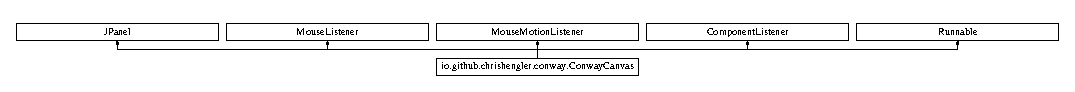
\includegraphics[height=0.788732cm]{classio_1_1github_1_1chrishengler_1_1conway_1_1_conway_canvas}
\end{center}
\end{figure}
\subsection*{Public Member Functions}
\begin{DoxyCompactItemize}
\item 
\hyperlink{classio_1_1github_1_1chrishengler_1_1conway_1_1_conway_canvas_a05e3fb830cb3bc30f6915dbdcf413e33}{Conway\+Canvas} (\hyperlink{classio_1_1github_1_1chrishengler_1_1conway_1_1_game}{Game} g)
\item 
\hyperlink{classio_1_1github_1_1chrishengler_1_1conway_1_1_game}{Game} \hyperlink{classio_1_1github_1_1chrishengler_1_1conway_1_1_conway_canvas_a8d0713b9676e81693a4f205359cbdd2c}{get\+Game} ()
\item 
Dimension \hyperlink{classio_1_1github_1_1chrishengler_1_1conway_1_1_conway_canvas_a372d17eeea7391a3db4194cafa321ed5}{get\+Preferred\+Size} ()
\item 
void \hyperlink{classio_1_1github_1_1chrishengler_1_1conway_1_1_conway_canvas_a4741c2dfc2913ba79e8e4218401a6c71}{paint\+Component} (Graphics g)
\item 
void \hyperlink{classio_1_1github_1_1chrishengler_1_1conway_1_1_conway_canvas_af573b11d5c693a94c605f0b6de1eea00}{mouse\+Released} (Mouse\+Event e)
\item 
void \hyperlink{classio_1_1github_1_1chrishengler_1_1conway_1_1_conway_canvas_a5e892360ad85e63435b65f55c6d67566}{mouse\+Dragged} (Mouse\+Event e)
\item 
void \hyperlink{classio_1_1github_1_1chrishengler_1_1conway_1_1_conway_canvas_a5b9c577520a81a80599ac9c591f678f6}{mouse\+Clicked} (Mouse\+Event e)
\item 
void \hyperlink{classio_1_1github_1_1chrishengler_1_1conway_1_1_conway_canvas_a9d2b3c6f5be5f2ab11c90b2658d3ab1d}{mouse\+Pressed} (Mouse\+Event e)
\item 
void \hyperlink{classio_1_1github_1_1chrishengler_1_1conway_1_1_conway_canvas_aab7389a32ac1f365ab26e6d68687fdcf}{mouse\+Entered} (Mouse\+Event e)
\item 
void \hyperlink{classio_1_1github_1_1chrishengler_1_1conway_1_1_conway_canvas_ad04a3ee8212500ccd023cc7ce20e9835}{mouse\+Exited} (Mouse\+Event e)
\item 
void \hyperlink{classio_1_1github_1_1chrishengler_1_1conway_1_1_conway_canvas_a82fe5a7bc1e656b73d22e8206310e97d}{mouse\+Moved} (Mouse\+Event e)
\item 
void \hyperlink{classio_1_1github_1_1chrishengler_1_1conway_1_1_conway_canvas_a7899d6724284cd68df5d4ea7b3c65c8b}{component\+Resized} (Component\+Event e)
\item 
void \hyperlink{classio_1_1github_1_1chrishengler_1_1conway_1_1_conway_canvas_a8e96f073d34272ea0fba93f41602411e}{component\+Moved} (Component\+Event e)
\item 
void \hyperlink{classio_1_1github_1_1chrishengler_1_1conway_1_1_conway_canvas_a6c512471e9814651ad1fd6ecb777e713}{component\+Shown} (Component\+Event e)
\item 
void \hyperlink{classio_1_1github_1_1chrishengler_1_1conway_1_1_conway_canvas_ad29ca955072daf022bca4303c1bb0a98}{component\+Hidden} (Component\+Event e)
\item 
void \hyperlink{classio_1_1github_1_1chrishengler_1_1conway_1_1_conway_canvas_a70f6dce6432c31a3532ef586df1d9420}{run} ()
\item 
void \hyperlink{classio_1_1github_1_1chrishengler_1_1conway_1_1_conway_canvas_a2f203de7f6ceca7ca93413bf7a4e9093}{set\+Step\+Time} (int time)
\end{DoxyCompactItemize}
\subsection*{Public Attributes}
\begin{DoxyCompactItemize}
\item 
boolean \hyperlink{classio_1_1github_1_1chrishengler_1_1conway_1_1_conway_canvas_acf462c13551f9c841d16cc960830ee7e}{m\+\_\+stop}
\end{DoxyCompactItemize}


\subsection{Detailed Description}
\begin{DoxyAuthor}{Author}
Chris Hengler 
\end{DoxyAuthor}


\subsection{Constructor \& Destructor Documentation}
\index{io\+::github\+::chrishengler\+::conway\+::\+Conway\+Canvas@{io\+::github\+::chrishengler\+::conway\+::\+Conway\+Canvas}!Conway\+Canvas@{Conway\+Canvas}}
\index{Conway\+Canvas@{Conway\+Canvas}!io\+::github\+::chrishengler\+::conway\+::\+Conway\+Canvas@{io\+::github\+::chrishengler\+::conway\+::\+Conway\+Canvas}}
\subsubsection[{\texorpdfstring{Conway\+Canvas(\+Game g)}{ConwayCanvas(Game g)}}]{\setlength{\rightskip}{0pt plus 5cm}io.\+github.\+chrishengler.\+conway.\+Conway\+Canvas.\+Conway\+Canvas (
\begin{DoxyParamCaption}
\item[{{\bf Game}}]{g}
\end{DoxyParamCaption}
)}\hypertarget{classio_1_1github_1_1chrishengler_1_1conway_1_1_conway_canvas_a05e3fb830cb3bc30f6915dbdcf413e33}{}\label{classio_1_1github_1_1chrishengler_1_1conway_1_1_conway_canvas_a05e3fb830cb3bc30f6915dbdcf413e33}
Creates new form \hyperlink{classio_1_1github_1_1chrishengler_1_1conway_1_1_conway_canvas}{Conway\+Canvas}


\begin{DoxyParams}{Parameters}
{\em g} & the \hyperlink{classio_1_1github_1_1chrishengler_1_1conway_1_1_game}{Game} we\textquotesingle{}ll be drawing \\
\hline
\end{DoxyParams}


\subsection{Member Function Documentation}
\index{io\+::github\+::chrishengler\+::conway\+::\+Conway\+Canvas@{io\+::github\+::chrishengler\+::conway\+::\+Conway\+Canvas}!component\+Hidden@{component\+Hidden}}
\index{component\+Hidden@{component\+Hidden}!io\+::github\+::chrishengler\+::conway\+::\+Conway\+Canvas@{io\+::github\+::chrishengler\+::conway\+::\+Conway\+Canvas}}
\subsubsection[{\texorpdfstring{component\+Hidden(\+Component\+Event e)}{componentHidden(ComponentEvent e)}}]{\setlength{\rightskip}{0pt plus 5cm}void io.\+github.\+chrishengler.\+conway.\+Conway\+Canvas.\+component\+Hidden (
\begin{DoxyParamCaption}
\item[{Component\+Event}]{e}
\end{DoxyParamCaption}
)}\hypertarget{classio_1_1github_1_1chrishengler_1_1conway_1_1_conway_canvas_ad29ca955072daf022bca4303c1bb0a98}{}\label{classio_1_1github_1_1chrishengler_1_1conway_1_1_conway_canvas_ad29ca955072daf022bca4303c1bb0a98}
\index{io\+::github\+::chrishengler\+::conway\+::\+Conway\+Canvas@{io\+::github\+::chrishengler\+::conway\+::\+Conway\+Canvas}!component\+Moved@{component\+Moved}}
\index{component\+Moved@{component\+Moved}!io\+::github\+::chrishengler\+::conway\+::\+Conway\+Canvas@{io\+::github\+::chrishengler\+::conway\+::\+Conway\+Canvas}}
\subsubsection[{\texorpdfstring{component\+Moved(\+Component\+Event e)}{componentMoved(ComponentEvent e)}}]{\setlength{\rightskip}{0pt plus 5cm}void io.\+github.\+chrishengler.\+conway.\+Conway\+Canvas.\+component\+Moved (
\begin{DoxyParamCaption}
\item[{Component\+Event}]{e}
\end{DoxyParamCaption}
)}\hypertarget{classio_1_1github_1_1chrishengler_1_1conway_1_1_conway_canvas_a8e96f073d34272ea0fba93f41602411e}{}\label{classio_1_1github_1_1chrishengler_1_1conway_1_1_conway_canvas_a8e96f073d34272ea0fba93f41602411e}
\index{io\+::github\+::chrishengler\+::conway\+::\+Conway\+Canvas@{io\+::github\+::chrishengler\+::conway\+::\+Conway\+Canvas}!component\+Resized@{component\+Resized}}
\index{component\+Resized@{component\+Resized}!io\+::github\+::chrishengler\+::conway\+::\+Conway\+Canvas@{io\+::github\+::chrishengler\+::conway\+::\+Conway\+Canvas}}
\subsubsection[{\texorpdfstring{component\+Resized(\+Component\+Event e)}{componentResized(ComponentEvent e)}}]{\setlength{\rightskip}{0pt plus 5cm}void io.\+github.\+chrishengler.\+conway.\+Conway\+Canvas.\+component\+Resized (
\begin{DoxyParamCaption}
\item[{Component\+Event}]{e}
\end{DoxyParamCaption}
)}\hypertarget{classio_1_1github_1_1chrishengler_1_1conway_1_1_conway_canvas_a7899d6724284cd68df5d4ea7b3c65c8b}{}\label{classio_1_1github_1_1chrishengler_1_1conway_1_1_conway_canvas_a7899d6724284cd68df5d4ea7b3c65c8b}
\index{io\+::github\+::chrishengler\+::conway\+::\+Conway\+Canvas@{io\+::github\+::chrishengler\+::conway\+::\+Conway\+Canvas}!component\+Shown@{component\+Shown}}
\index{component\+Shown@{component\+Shown}!io\+::github\+::chrishengler\+::conway\+::\+Conway\+Canvas@{io\+::github\+::chrishengler\+::conway\+::\+Conway\+Canvas}}
\subsubsection[{\texorpdfstring{component\+Shown(\+Component\+Event e)}{componentShown(ComponentEvent e)}}]{\setlength{\rightskip}{0pt plus 5cm}void io.\+github.\+chrishengler.\+conway.\+Conway\+Canvas.\+component\+Shown (
\begin{DoxyParamCaption}
\item[{Component\+Event}]{e}
\end{DoxyParamCaption}
)}\hypertarget{classio_1_1github_1_1chrishengler_1_1conway_1_1_conway_canvas_a6c512471e9814651ad1fd6ecb777e713}{}\label{classio_1_1github_1_1chrishengler_1_1conway_1_1_conway_canvas_a6c512471e9814651ad1fd6ecb777e713}
\index{io\+::github\+::chrishengler\+::conway\+::\+Conway\+Canvas@{io\+::github\+::chrishengler\+::conway\+::\+Conway\+Canvas}!get\+Game@{get\+Game}}
\index{get\+Game@{get\+Game}!io\+::github\+::chrishengler\+::conway\+::\+Conway\+Canvas@{io\+::github\+::chrishengler\+::conway\+::\+Conway\+Canvas}}
\subsubsection[{\texorpdfstring{get\+Game()}{getGame()}}]{\setlength{\rightskip}{0pt plus 5cm}{\bf Game} io.\+github.\+chrishengler.\+conway.\+Conway\+Canvas.\+get\+Game (
\begin{DoxyParamCaption}
{}
\end{DoxyParamCaption}
)}\hypertarget{classio_1_1github_1_1chrishengler_1_1conway_1_1_conway_canvas_a8d0713b9676e81693a4f205359cbdd2c}{}\label{classio_1_1github_1_1chrishengler_1_1conway_1_1_conway_canvas_a8d0713b9676e81693a4f205359cbdd2c}
return \hyperlink{classio_1_1github_1_1chrishengler_1_1conway_1_1_game}{Game} m\+\_\+game

\begin{DoxyReturn}{Returns}
m\+\_\+game 
\end{DoxyReturn}
\index{io\+::github\+::chrishengler\+::conway\+::\+Conway\+Canvas@{io\+::github\+::chrishengler\+::conway\+::\+Conway\+Canvas}!get\+Preferred\+Size@{get\+Preferred\+Size}}
\index{get\+Preferred\+Size@{get\+Preferred\+Size}!io\+::github\+::chrishengler\+::conway\+::\+Conway\+Canvas@{io\+::github\+::chrishengler\+::conway\+::\+Conway\+Canvas}}
\subsubsection[{\texorpdfstring{get\+Preferred\+Size()}{getPreferredSize()}}]{\setlength{\rightskip}{0pt plus 5cm}Dimension io.\+github.\+chrishengler.\+conway.\+Conway\+Canvas.\+get\+Preferred\+Size (
\begin{DoxyParamCaption}
{}
\end{DoxyParamCaption}
)}\hypertarget{classio_1_1github_1_1chrishengler_1_1conway_1_1_conway_canvas_a372d17eeea7391a3db4194cafa321ed5}{}\label{classio_1_1github_1_1chrishengler_1_1conway_1_1_conway_canvas_a372d17eeea7391a3db4194cafa321ed5}
\index{io\+::github\+::chrishengler\+::conway\+::\+Conway\+Canvas@{io\+::github\+::chrishengler\+::conway\+::\+Conway\+Canvas}!mouse\+Clicked@{mouse\+Clicked}}
\index{mouse\+Clicked@{mouse\+Clicked}!io\+::github\+::chrishengler\+::conway\+::\+Conway\+Canvas@{io\+::github\+::chrishengler\+::conway\+::\+Conway\+Canvas}}
\subsubsection[{\texorpdfstring{mouse\+Clicked(\+Mouse\+Event e)}{mouseClicked(MouseEvent e)}}]{\setlength{\rightskip}{0pt plus 5cm}void io.\+github.\+chrishengler.\+conway.\+Conway\+Canvas.\+mouse\+Clicked (
\begin{DoxyParamCaption}
\item[{Mouse\+Event}]{e}
\end{DoxyParamCaption}
)}\hypertarget{classio_1_1github_1_1chrishengler_1_1conway_1_1_conway_canvas_a5b9c577520a81a80599ac9c591f678f6}{}\label{classio_1_1github_1_1chrishengler_1_1conway_1_1_conway_canvas_a5b9c577520a81a80599ac9c591f678f6}
\index{io\+::github\+::chrishengler\+::conway\+::\+Conway\+Canvas@{io\+::github\+::chrishengler\+::conway\+::\+Conway\+Canvas}!mouse\+Dragged@{mouse\+Dragged}}
\index{mouse\+Dragged@{mouse\+Dragged}!io\+::github\+::chrishengler\+::conway\+::\+Conway\+Canvas@{io\+::github\+::chrishengler\+::conway\+::\+Conway\+Canvas}}
\subsubsection[{\texorpdfstring{mouse\+Dragged(\+Mouse\+Event e)}{mouseDragged(MouseEvent e)}}]{\setlength{\rightskip}{0pt plus 5cm}void io.\+github.\+chrishengler.\+conway.\+Conway\+Canvas.\+mouse\+Dragged (
\begin{DoxyParamCaption}
\item[{Mouse\+Event}]{e}
\end{DoxyParamCaption}
)}\hypertarget{classio_1_1github_1_1chrishengler_1_1conway_1_1_conway_canvas_a5e892360ad85e63435b65f55c6d67566}{}\label{classio_1_1github_1_1chrishengler_1_1conway_1_1_conway_canvas_a5e892360ad85e63435b65f55c6d67566}
\index{io\+::github\+::chrishengler\+::conway\+::\+Conway\+Canvas@{io\+::github\+::chrishengler\+::conway\+::\+Conway\+Canvas}!mouse\+Entered@{mouse\+Entered}}
\index{mouse\+Entered@{mouse\+Entered}!io\+::github\+::chrishengler\+::conway\+::\+Conway\+Canvas@{io\+::github\+::chrishengler\+::conway\+::\+Conway\+Canvas}}
\subsubsection[{\texorpdfstring{mouse\+Entered(\+Mouse\+Event e)}{mouseEntered(MouseEvent e)}}]{\setlength{\rightskip}{0pt plus 5cm}void io.\+github.\+chrishengler.\+conway.\+Conway\+Canvas.\+mouse\+Entered (
\begin{DoxyParamCaption}
\item[{Mouse\+Event}]{e}
\end{DoxyParamCaption}
)}\hypertarget{classio_1_1github_1_1chrishengler_1_1conway_1_1_conway_canvas_aab7389a32ac1f365ab26e6d68687fdcf}{}\label{classio_1_1github_1_1chrishengler_1_1conway_1_1_conway_canvas_aab7389a32ac1f365ab26e6d68687fdcf}
\index{io\+::github\+::chrishengler\+::conway\+::\+Conway\+Canvas@{io\+::github\+::chrishengler\+::conway\+::\+Conway\+Canvas}!mouse\+Exited@{mouse\+Exited}}
\index{mouse\+Exited@{mouse\+Exited}!io\+::github\+::chrishengler\+::conway\+::\+Conway\+Canvas@{io\+::github\+::chrishengler\+::conway\+::\+Conway\+Canvas}}
\subsubsection[{\texorpdfstring{mouse\+Exited(\+Mouse\+Event e)}{mouseExited(MouseEvent e)}}]{\setlength{\rightskip}{0pt plus 5cm}void io.\+github.\+chrishengler.\+conway.\+Conway\+Canvas.\+mouse\+Exited (
\begin{DoxyParamCaption}
\item[{Mouse\+Event}]{e}
\end{DoxyParamCaption}
)}\hypertarget{classio_1_1github_1_1chrishengler_1_1conway_1_1_conway_canvas_ad04a3ee8212500ccd023cc7ce20e9835}{}\label{classio_1_1github_1_1chrishengler_1_1conway_1_1_conway_canvas_ad04a3ee8212500ccd023cc7ce20e9835}
\index{io\+::github\+::chrishengler\+::conway\+::\+Conway\+Canvas@{io\+::github\+::chrishengler\+::conway\+::\+Conway\+Canvas}!mouse\+Moved@{mouse\+Moved}}
\index{mouse\+Moved@{mouse\+Moved}!io\+::github\+::chrishengler\+::conway\+::\+Conway\+Canvas@{io\+::github\+::chrishengler\+::conway\+::\+Conway\+Canvas}}
\subsubsection[{\texorpdfstring{mouse\+Moved(\+Mouse\+Event e)}{mouseMoved(MouseEvent e)}}]{\setlength{\rightskip}{0pt plus 5cm}void io.\+github.\+chrishengler.\+conway.\+Conway\+Canvas.\+mouse\+Moved (
\begin{DoxyParamCaption}
\item[{Mouse\+Event}]{e}
\end{DoxyParamCaption}
)}\hypertarget{classio_1_1github_1_1chrishengler_1_1conway_1_1_conway_canvas_a82fe5a7bc1e656b73d22e8206310e97d}{}\label{classio_1_1github_1_1chrishengler_1_1conway_1_1_conway_canvas_a82fe5a7bc1e656b73d22e8206310e97d}
\index{io\+::github\+::chrishengler\+::conway\+::\+Conway\+Canvas@{io\+::github\+::chrishengler\+::conway\+::\+Conway\+Canvas}!mouse\+Pressed@{mouse\+Pressed}}
\index{mouse\+Pressed@{mouse\+Pressed}!io\+::github\+::chrishengler\+::conway\+::\+Conway\+Canvas@{io\+::github\+::chrishengler\+::conway\+::\+Conway\+Canvas}}
\subsubsection[{\texorpdfstring{mouse\+Pressed(\+Mouse\+Event e)}{mousePressed(MouseEvent e)}}]{\setlength{\rightskip}{0pt plus 5cm}void io.\+github.\+chrishengler.\+conway.\+Conway\+Canvas.\+mouse\+Pressed (
\begin{DoxyParamCaption}
\item[{Mouse\+Event}]{e}
\end{DoxyParamCaption}
)}\hypertarget{classio_1_1github_1_1chrishengler_1_1conway_1_1_conway_canvas_a9d2b3c6f5be5f2ab11c90b2658d3ab1d}{}\label{classio_1_1github_1_1chrishengler_1_1conway_1_1_conway_canvas_a9d2b3c6f5be5f2ab11c90b2658d3ab1d}
\index{io\+::github\+::chrishengler\+::conway\+::\+Conway\+Canvas@{io\+::github\+::chrishengler\+::conway\+::\+Conway\+Canvas}!mouse\+Released@{mouse\+Released}}
\index{mouse\+Released@{mouse\+Released}!io\+::github\+::chrishengler\+::conway\+::\+Conway\+Canvas@{io\+::github\+::chrishengler\+::conway\+::\+Conway\+Canvas}}
\subsubsection[{\texorpdfstring{mouse\+Released(\+Mouse\+Event e)}{mouseReleased(MouseEvent e)}}]{\setlength{\rightskip}{0pt plus 5cm}void io.\+github.\+chrishengler.\+conway.\+Conway\+Canvas.\+mouse\+Released (
\begin{DoxyParamCaption}
\item[{Mouse\+Event}]{e}
\end{DoxyParamCaption}
)}\hypertarget{classio_1_1github_1_1chrishengler_1_1conway_1_1_conway_canvas_af573b11d5c693a94c605f0b6de1eea00}{}\label{classio_1_1github_1_1chrishengler_1_1conway_1_1_conway_canvas_af573b11d5c693a94c605f0b6de1eea00}
\index{io\+::github\+::chrishengler\+::conway\+::\+Conway\+Canvas@{io\+::github\+::chrishengler\+::conway\+::\+Conway\+Canvas}!paint\+Component@{paint\+Component}}
\index{paint\+Component@{paint\+Component}!io\+::github\+::chrishengler\+::conway\+::\+Conway\+Canvas@{io\+::github\+::chrishengler\+::conway\+::\+Conway\+Canvas}}
\subsubsection[{\texorpdfstring{paint\+Component(\+Graphics g)}{paintComponent(Graphics g)}}]{\setlength{\rightskip}{0pt plus 5cm}void io.\+github.\+chrishengler.\+conway.\+Conway\+Canvas.\+paint\+Component (
\begin{DoxyParamCaption}
\item[{Graphics}]{g}
\end{DoxyParamCaption}
)}\hypertarget{classio_1_1github_1_1chrishengler_1_1conway_1_1_conway_canvas_a4741c2dfc2913ba79e8e4218401a6c71}{}\label{classio_1_1github_1_1chrishengler_1_1conway_1_1_conway_canvas_a4741c2dfc2913ba79e8e4218401a6c71}
\index{io\+::github\+::chrishengler\+::conway\+::\+Conway\+Canvas@{io\+::github\+::chrishengler\+::conway\+::\+Conway\+Canvas}!run@{run}}
\index{run@{run}!io\+::github\+::chrishengler\+::conway\+::\+Conway\+Canvas@{io\+::github\+::chrishengler\+::conway\+::\+Conway\+Canvas}}
\subsubsection[{\texorpdfstring{run()}{run()}}]{\setlength{\rightskip}{0pt plus 5cm}void io.\+github.\+chrishengler.\+conway.\+Conway\+Canvas.\+run (
\begin{DoxyParamCaption}
{}
\end{DoxyParamCaption}
)}\hypertarget{classio_1_1github_1_1chrishengler_1_1conway_1_1_conway_canvas_a70f6dce6432c31a3532ef586df1d9420}{}\label{classio_1_1github_1_1chrishengler_1_1conway_1_1_conway_canvas_a70f6dce6432c31a3532ef586df1d9420}
\index{io\+::github\+::chrishengler\+::conway\+::\+Conway\+Canvas@{io\+::github\+::chrishengler\+::conway\+::\+Conway\+Canvas}!set\+Step\+Time@{set\+Step\+Time}}
\index{set\+Step\+Time@{set\+Step\+Time}!io\+::github\+::chrishengler\+::conway\+::\+Conway\+Canvas@{io\+::github\+::chrishengler\+::conway\+::\+Conway\+Canvas}}
\subsubsection[{\texorpdfstring{set\+Step\+Time(int time)}{setStepTime(int time)}}]{\setlength{\rightskip}{0pt plus 5cm}void io.\+github.\+chrishengler.\+conway.\+Conway\+Canvas.\+set\+Step\+Time (
\begin{DoxyParamCaption}
\item[{int}]{time}
\end{DoxyParamCaption}
)}\hypertarget{classio_1_1github_1_1chrishengler_1_1conway_1_1_conway_canvas_a2f203de7f6ceca7ca93413bf7a4e9093}{}\label{classio_1_1github_1_1chrishengler_1_1conway_1_1_conway_canvas_a2f203de7f6ceca7ca93413bf7a4e9093}
set time between steps in ms


\begin{DoxyParams}{Parameters}
{\em time} & delay in ms beween iterations \\
\hline
\end{DoxyParams}


\subsection{Member Data Documentation}
\index{io\+::github\+::chrishengler\+::conway\+::\+Conway\+Canvas@{io\+::github\+::chrishengler\+::conway\+::\+Conway\+Canvas}!m\+\_\+stop@{m\+\_\+stop}}
\index{m\+\_\+stop@{m\+\_\+stop}!io\+::github\+::chrishengler\+::conway\+::\+Conway\+Canvas@{io\+::github\+::chrishengler\+::conway\+::\+Conway\+Canvas}}
\subsubsection[{\texorpdfstring{m\+\_\+stop}{m\_stop}}]{\setlength{\rightskip}{0pt plus 5cm}boolean io.\+github.\+chrishengler.\+conway.\+Conway\+Canvas.\+m\+\_\+stop}\hypertarget{classio_1_1github_1_1chrishengler_1_1conway_1_1_conway_canvas_acf462c13551f9c841d16cc960830ee7e}{}\label{classio_1_1github_1_1chrishengler_1_1conway_1_1_conway_canvas_acf462c13551f9c841d16cc960830ee7e}
used as trigger to stop running game in background thread 

The documentation for this class was generated from the following file\+:\begin{DoxyCompactItemize}
\item 
io/github/chrishengler/conway/Conway\+Canvas.\+java\end{DoxyCompactItemize}

\hypertarget{classio_1_1github_1_1chrishengler_1_1conway_1_1_game}{}\section{io.\+github.\+chrishengler.\+conway.\+Game Class Reference}
\label{classio_1_1github_1_1chrishengler_1_1conway_1_1_game}\index{io.\+github.\+chrishengler.\+conway.\+Game@{io.\+github.\+chrishengler.\+conway.\+Game}}
\subsection*{Public Member Functions}
\begin{DoxyCompactItemize}
\item 
\hyperlink{classio_1_1github_1_1chrishengler_1_1conway_1_1_game_ad1fc4a4831375c08da54f3ed5ea86497}{Game} ()
\item 
\hyperlink{classio_1_1github_1_1chrishengler_1_1conway_1_1_game_a3cac815fa6b8c5e753accc9930068801}{Game} (int x, int y)
\item 
\hyperlink{classio_1_1github_1_1chrishengler_1_1conway_1_1_game_af99bec40d23e8207f974933989721740}{Game} (int x, int y, \hyperlink{classio_1_1github_1_1chrishengler_1_1conway_1_1_game}{Game} g)
\item 
void \hyperlink{classio_1_1github_1_1chrishengler_1_1conway_1_1_game_aa906c1d00d7dd8bf267ba10206d3465e}{resize\+Board} (int x, int y)
\item 
void \hyperlink{classio_1_1github_1_1chrishengler_1_1conway_1_1_game_aa6b4e9095b28f2f9fe10410089b7570b}{fill\+Random} (double p)
\item 
void \hyperlink{classio_1_1github_1_1chrishengler_1_1conway_1_1_game_ad82729652ed2d593324db51b0f6d49e7}{next\+Step} ()
\item 
\hyperlink{classio_1_1github_1_1chrishengler_1_1conway_1_1_cell_board}{Cell\+Board} \hyperlink{classio_1_1github_1_1chrishengler_1_1conway_1_1_game_a4ff5851c957ee998017f7f0911228a16}{get\+Board} ()
\item 
void \hyperlink{classio_1_1github_1_1chrishengler_1_1conway_1_1_game_a97e618d6f05f708c09b3f1c0c1b98c43}{set\+Alive} (int x, int y, boolean alive)
\item 
void \hyperlink{classio_1_1github_1_1chrishengler_1_1conway_1_1_game_aeb5f11f00e46a6471e813c7e2f951291}{toggle\+Cell} (int x, int y)
\item 
boolean \hyperlink{classio_1_1github_1_1chrishengler_1_1conway_1_1_game_ab26b20a57e7c46e105d9a881fa53cc31}{is\+Alive} (int x, int y)
\item 
int \hyperlink{classio_1_1github_1_1chrishengler_1_1conway_1_1_game_a7b6afc4b174fd150ddd9a053cfebc121}{getX} ()
\item 
int \hyperlink{classio_1_1github_1_1chrishengler_1_1conway_1_1_game_a43296dab4be1ce47cf2e1dffda221734}{getY} ()
\end{DoxyCompactItemize}


\subsection{Detailed Description}
\begin{DoxyAuthor}{Author}
Chris Hengler 
\end{DoxyAuthor}


\subsection{Constructor \& Destructor Documentation}
\index{io\+::github\+::chrishengler\+::conway\+::\+Game@{io\+::github\+::chrishengler\+::conway\+::\+Game}!Game@{Game}}
\index{Game@{Game}!io\+::github\+::chrishengler\+::conway\+::\+Game@{io\+::github\+::chrishengler\+::conway\+::\+Game}}
\subsubsection[{\texorpdfstring{Game()}{Game()}}]{\setlength{\rightskip}{0pt plus 5cm}io.\+github.\+chrishengler.\+conway.\+Game.\+Game (
\begin{DoxyParamCaption}
{}
\end{DoxyParamCaption}
)}\hypertarget{classio_1_1github_1_1chrishengler_1_1conway_1_1_game_ad1fc4a4831375c08da54f3ed5ea86497}{}\label{classio_1_1github_1_1chrishengler_1_1conway_1_1_game_ad1fc4a4831375c08da54f3ed5ea86497}
no-\/arg constructor, default size from \hyperlink{classio_1_1github_1_1chrishengler_1_1conway_1_1_cell_board}{Cell\+Board} \index{io\+::github\+::chrishengler\+::conway\+::\+Game@{io\+::github\+::chrishengler\+::conway\+::\+Game}!Game@{Game}}
\index{Game@{Game}!io\+::github\+::chrishengler\+::conway\+::\+Game@{io\+::github\+::chrishengler\+::conway\+::\+Game}}
\subsubsection[{\texorpdfstring{Game(int x, int y)}{Game(int x, int y)}}]{\setlength{\rightskip}{0pt plus 5cm}io.\+github.\+chrishengler.\+conway.\+Game.\+Game (
\begin{DoxyParamCaption}
\item[{int}]{x, }
\item[{int}]{y}
\end{DoxyParamCaption}
)}\hypertarget{classio_1_1github_1_1chrishengler_1_1conway_1_1_game_a3cac815fa6b8c5e753accc9930068801}{}\label{classio_1_1github_1_1chrishengler_1_1conway_1_1_game_a3cac815fa6b8c5e753accc9930068801}
constructor with x, y dimensions specified


\begin{DoxyParams}{Parameters}
{\em x} & \\
\hline
{\em y} & \\
\hline
\end{DoxyParams}
\index{io\+::github\+::chrishengler\+::conway\+::\+Game@{io\+::github\+::chrishengler\+::conway\+::\+Game}!Game@{Game}}
\index{Game@{Game}!io\+::github\+::chrishengler\+::conway\+::\+Game@{io\+::github\+::chrishengler\+::conway\+::\+Game}}
\subsubsection[{\texorpdfstring{Game(int x, int y, Game g)}{Game(int x, int y, Game g)}}]{\setlength{\rightskip}{0pt plus 5cm}io.\+github.\+chrishengler.\+conway.\+Game.\+Game (
\begin{DoxyParamCaption}
\item[{int}]{x, }
\item[{int}]{y, }
\item[{{\bf Game}}]{g}
\end{DoxyParamCaption}
)}\hypertarget{classio_1_1github_1_1chrishengler_1_1conway_1_1_game_af99bec40d23e8207f974933989721740}{}\label{classio_1_1github_1_1chrishengler_1_1conway_1_1_game_af99bec40d23e8207f974933989721740}
constructor with x,y dimensions specified and board populated 
\begin{DoxyParams}{Parameters}
{\em x} & \\
\hline
{\em y} & \\
\hline
{\em g} & \\
\hline
\end{DoxyParams}


\subsection{Member Function Documentation}
\index{io\+::github\+::chrishengler\+::conway\+::\+Game@{io\+::github\+::chrishengler\+::conway\+::\+Game}!fill\+Random@{fill\+Random}}
\index{fill\+Random@{fill\+Random}!io\+::github\+::chrishengler\+::conway\+::\+Game@{io\+::github\+::chrishengler\+::conway\+::\+Game}}
\subsubsection[{\texorpdfstring{fill\+Random(double p)}{fillRandom(double p)}}]{\setlength{\rightskip}{0pt plus 5cm}void io.\+github.\+chrishengler.\+conway.\+Game.\+fill\+Random (
\begin{DoxyParamCaption}
\item[{double}]{p}
\end{DoxyParamCaption}
)}\hypertarget{classio_1_1github_1_1chrishengler_1_1conway_1_1_game_aa6b4e9095b28f2f9fe10410089b7570b}{}\label{classio_1_1github_1_1chrishengler_1_1conway_1_1_game_aa6b4e9095b28f2f9fe10410089b7570b}
fill board randomly

Fill the board randomly. Each cell has probability p of being set to alive p is fractional probability, so should be in range 0 ≤ p ≤ 1


\begin{DoxyParams}{Parameters}
{\em p} & fraction of board to fill \\
\hline
\end{DoxyParams}
\index{io\+::github\+::chrishengler\+::conway\+::\+Game@{io\+::github\+::chrishengler\+::conway\+::\+Game}!get\+Board@{get\+Board}}
\index{get\+Board@{get\+Board}!io\+::github\+::chrishengler\+::conway\+::\+Game@{io\+::github\+::chrishengler\+::conway\+::\+Game}}
\subsubsection[{\texorpdfstring{get\+Board()}{getBoard()}}]{\setlength{\rightskip}{0pt plus 5cm}{\bf Cell\+Board} io.\+github.\+chrishengler.\+conway.\+Game.\+get\+Board (
\begin{DoxyParamCaption}
{}
\end{DoxyParamCaption}
)}\hypertarget{classio_1_1github_1_1chrishengler_1_1conway_1_1_game_a4ff5851c957ee998017f7f0911228a16}{}\label{classio_1_1github_1_1chrishengler_1_1conway_1_1_game_a4ff5851c957ee998017f7f0911228a16}
return game\textquotesingle{}s \hyperlink{classio_1_1github_1_1chrishengler_1_1conway_1_1_cell_board}{Cell\+Board} (m\+\_\+board)

\begin{DoxyReturn}{Returns}
\hyperlink{classio_1_1github_1_1chrishengler_1_1conway_1_1_cell_board}{Cell\+Board} m\+\_\+board 
\end{DoxyReturn}
\index{io\+::github\+::chrishengler\+::conway\+::\+Game@{io\+::github\+::chrishengler\+::conway\+::\+Game}!getX@{getX}}
\index{getX@{getX}!io\+::github\+::chrishengler\+::conway\+::\+Game@{io\+::github\+::chrishengler\+::conway\+::\+Game}}
\subsubsection[{\texorpdfstring{get\+X()}{getX()}}]{\setlength{\rightskip}{0pt plus 5cm}int io.\+github.\+chrishengler.\+conway.\+Game.\+getX (
\begin{DoxyParamCaption}
{}
\end{DoxyParamCaption}
)}\hypertarget{classio_1_1github_1_1chrishengler_1_1conway_1_1_game_a7b6afc4b174fd150ddd9a053cfebc121}{}\label{classio_1_1github_1_1chrishengler_1_1conway_1_1_game_a7b6afc4b174fd150ddd9a053cfebc121}
get number of columns in board

\begin{DoxyReturn}{Returns}
number of columns 
\end{DoxyReturn}
\index{io\+::github\+::chrishengler\+::conway\+::\+Game@{io\+::github\+::chrishengler\+::conway\+::\+Game}!getY@{getY}}
\index{getY@{getY}!io\+::github\+::chrishengler\+::conway\+::\+Game@{io\+::github\+::chrishengler\+::conway\+::\+Game}}
\subsubsection[{\texorpdfstring{get\+Y()}{getY()}}]{\setlength{\rightskip}{0pt plus 5cm}int io.\+github.\+chrishengler.\+conway.\+Game.\+getY (
\begin{DoxyParamCaption}
{}
\end{DoxyParamCaption}
)}\hypertarget{classio_1_1github_1_1chrishengler_1_1conway_1_1_game_a43296dab4be1ce47cf2e1dffda221734}{}\label{classio_1_1github_1_1chrishengler_1_1conway_1_1_game_a43296dab4be1ce47cf2e1dffda221734}
get number of rows in board

\begin{DoxyReturn}{Returns}
number of rows 
\end{DoxyReturn}
\index{io\+::github\+::chrishengler\+::conway\+::\+Game@{io\+::github\+::chrishengler\+::conway\+::\+Game}!is\+Alive@{is\+Alive}}
\index{is\+Alive@{is\+Alive}!io\+::github\+::chrishengler\+::conway\+::\+Game@{io\+::github\+::chrishengler\+::conway\+::\+Game}}
\subsubsection[{\texorpdfstring{is\+Alive(int x, int y)}{isAlive(int x, int y)}}]{\setlength{\rightskip}{0pt plus 5cm}boolean io.\+github.\+chrishengler.\+conway.\+Game.\+is\+Alive (
\begin{DoxyParamCaption}
\item[{int}]{x, }
\item[{int}]{y}
\end{DoxyParamCaption}
)}\hypertarget{classio_1_1github_1_1chrishengler_1_1conway_1_1_game_ab26b20a57e7c46e105d9a881fa53cc31}{}\label{classio_1_1github_1_1chrishengler_1_1conway_1_1_game_ab26b20a57e7c46e105d9a881fa53cc31}
calls Cell\+Board.\+is\+Alive(x,y);


\begin{DoxyParams}{Parameters}
{\em x} & \\
\hline
{\em y} & \\
\hline
\end{DoxyParams}
\begin{DoxyReturn}{Returns}

\end{DoxyReturn}
\index{io\+::github\+::chrishengler\+::conway\+::\+Game@{io\+::github\+::chrishengler\+::conway\+::\+Game}!next\+Step@{next\+Step}}
\index{next\+Step@{next\+Step}!io\+::github\+::chrishengler\+::conway\+::\+Game@{io\+::github\+::chrishengler\+::conway\+::\+Game}}
\subsubsection[{\texorpdfstring{next\+Step()}{nextStep()}}]{\setlength{\rightskip}{0pt plus 5cm}void io.\+github.\+chrishengler.\+conway.\+Game.\+next\+Step (
\begin{DoxyParamCaption}
{}
\end{DoxyParamCaption}
)}\hypertarget{classio_1_1github_1_1chrishengler_1_1conway_1_1_game_ad82729652ed2d593324db51b0f6d49e7}{}\label{classio_1_1github_1_1chrishengler_1_1conway_1_1_game_ad82729652ed2d593324db51b0f6d49e7}
update game status to next step \index{io\+::github\+::chrishengler\+::conway\+::\+Game@{io\+::github\+::chrishengler\+::conway\+::\+Game}!resize\+Board@{resize\+Board}}
\index{resize\+Board@{resize\+Board}!io\+::github\+::chrishengler\+::conway\+::\+Game@{io\+::github\+::chrishengler\+::conway\+::\+Game}}
\subsubsection[{\texorpdfstring{resize\+Board(int x, int y)}{resizeBoard(int x, int y)}}]{\setlength{\rightskip}{0pt plus 5cm}void io.\+github.\+chrishengler.\+conway.\+Game.\+resize\+Board (
\begin{DoxyParamCaption}
\item[{int}]{x, }
\item[{int}]{y}
\end{DoxyParamCaption}
)}\hypertarget{classio_1_1github_1_1chrishengler_1_1conway_1_1_game_aa906c1d00d7dd8bf267ba10206d3465e}{}\label{classio_1_1github_1_1chrishengler_1_1conway_1_1_game_aa906c1d00d7dd8bf267ba10206d3465e}
resize board to have size (in cells) x,y


\begin{DoxyParams}{Parameters}
{\em x} & \\
\hline
{\em y} & \\
\hline
\end{DoxyParams}
\index{io\+::github\+::chrishengler\+::conway\+::\+Game@{io\+::github\+::chrishengler\+::conway\+::\+Game}!set\+Alive@{set\+Alive}}
\index{set\+Alive@{set\+Alive}!io\+::github\+::chrishengler\+::conway\+::\+Game@{io\+::github\+::chrishengler\+::conway\+::\+Game}}
\subsubsection[{\texorpdfstring{set\+Alive(int x, int y, boolean alive)}{setAlive(int x, int y, boolean alive)}}]{\setlength{\rightskip}{0pt plus 5cm}void io.\+github.\+chrishengler.\+conway.\+Game.\+set\+Alive (
\begin{DoxyParamCaption}
\item[{int}]{x, }
\item[{int}]{y, }
\item[{boolean}]{alive}
\end{DoxyParamCaption}
)}\hypertarget{classio_1_1github_1_1chrishengler_1_1conway_1_1_game_a97e618d6f05f708c09b3f1c0c1b98c43}{}\label{classio_1_1github_1_1chrishengler_1_1conway_1_1_game_a97e618d6f05f708c09b3f1c0c1b98c43}
calls Cell\+Board.\+set\+Alive(x,y,alive);


\begin{DoxyParams}{Parameters}
{\em x} & \\
\hline
{\em y} & \\
\hline
{\em alive} & \\
\hline
\end{DoxyParams}
\index{io\+::github\+::chrishengler\+::conway\+::\+Game@{io\+::github\+::chrishengler\+::conway\+::\+Game}!toggle\+Cell@{toggle\+Cell}}
\index{toggle\+Cell@{toggle\+Cell}!io\+::github\+::chrishengler\+::conway\+::\+Game@{io\+::github\+::chrishengler\+::conway\+::\+Game}}
\subsubsection[{\texorpdfstring{toggle\+Cell(int x, int y)}{toggleCell(int x, int y)}}]{\setlength{\rightskip}{0pt plus 5cm}void io.\+github.\+chrishengler.\+conway.\+Game.\+toggle\+Cell (
\begin{DoxyParamCaption}
\item[{int}]{x, }
\item[{int}]{y}
\end{DoxyParamCaption}
)}\hypertarget{classio_1_1github_1_1chrishengler_1_1conway_1_1_game_aeb5f11f00e46a6471e813c7e2f951291}{}\label{classio_1_1github_1_1chrishengler_1_1conway_1_1_game_aeb5f11f00e46a6471e813c7e2f951291}
calls Cell\+Board.\+toggle\+Cell(x,y);


\begin{DoxyParams}{Parameters}
{\em x} & \\
\hline
{\em y} & \\
\hline
\end{DoxyParams}


The documentation for this class was generated from the following file\+:\begin{DoxyCompactItemize}
\item 
io/github/chrishengler/conway/Game.\+java\end{DoxyCompactItemize}

%--- End generated contents ---

% Index
\backmatter
\newpage
\phantomsection
\clearemptydoublepage
\addcontentsline{toc}{chapter}{Index}
\printindex

\end{document}
